% main.tex --- 修論用アブスト（2ページ二段組, LuaLaTeX）
\documentclass[a4paper,10pt,twocolumn]{ltjsarticle}

\usepackage[haranoaji]{luatexja-preset}
\usepackage[top=17mm,bottom=17mm,left=17mm,right=17mm]{geometry}
\usepackage{graphicx}
\usepackage{booktabs}
\usepackage{siunitx}
\usepackage{caption}
\usepackage{capt-of}
\usepackage{titlesec}
\usepackage{multicol}
\usepackage{amsmath}
\usepackage[hidelinks]{hyperref}
\usepackage[
  backend=biber,
  style=numeric,
  sorting=none,
  maxnames=3,
  minnames=1,
  giveninits=true,
  doi=false,
  url=false,
  isbn=false,
  eprint=false
]{biblatex}

% meta.tex --- 修論用アブスト（先頭ブロック用）

\newcommand{\AbstTitle}{QoS 制約下におけるHAR 不確実度に基づくBLE アドバタイジング間隔の適応制御}
\newcommand{\AbstAuthor}{萩原 圭島}
\newcommand{\AbstAdvisor}{木村 秀明}
\newcommand{\AbstAffiliation}{中部大学大学院 工学研究科 情報工学専攻}


\addbibresource{references.bib}

\pagestyle{empty}
\setlength{\columnsep}{5mm}
\setlength{\parindent}{1\zw}
\setlength{\parskip}{0pt}

\titleformat{\section}[runin]{\normalfont\normalsize\bfseries}{\thesection.}{0.5em}{}
\titlespacing*{\section}{0pt}{0.5\baselineskip}{1.2\zw}
\titleformat{\subsection}{\normalfont\small\bfseries}{\thesubsection}{0.5em}{}
\titlespacing*{\subsection}{0pt}{0.3\baselineskip}{0.1\baselineskip}

\DeclareCaptionLabelFormat{nonspace}{#1#2}
\captionsetup{labelformat=nonspace,labelsep=space}
\captionsetup[figure]{name=図,position=bottom}
\captionsetup[table]{name=表,position=top}
\captionsetup{skip=1pt}
\captionsetup{font=small}

\newcommand{\figref}[1]{図~\ref{#1}}
\newcommand{\tabref}[1]{表~\ref{#1}}
\newcommand{\Pout}{P_{\mathrm{out}}}
\newcommand{\epsout}{\epsilon}

\DeclareCiteCommand{\cite}
  {}
  {\mkbibbrackets{\usebibmacro{citeindex}\usebibmacro{cite}}}
  {}
  {}

\setlength{\textfloatsep}{2pt plus 1pt minus 1pt}
\setlength{\intextsep}{2pt plus 1pt minus 1pt}
\setlength{\floatsep}{2pt plus 1pt minus 1pt}
\setlength{\dbltextfloatsep}{2pt plus 1pt minus 1pt}
\setlength{\dblfloatsep}{2pt plus 1pt minus 1pt}

\renewcommand*{\bibfont}{\normalfont\small}
\setlength{\bibitemsep}{0pt}
\setlength{\bibparsep}{0pt}

\begin{document}

\twocolumn[
\begin{center}
  {\normalsize \AbstTitle\par}
  \vspace{0.5mm}
  {\small \AbstAuthor\quad \AbstAdvisor\par}
  {\small \AbstAffiliation\par}
  \vspace{2mm}
\end{center}
]

\section{はじめに}
見守りシステムにおいて，ウェアラブル端末による人間活動認識（HAR）の常時通信は電力消費の主要因である\cite{Luo2021BLENeighborDiscoverySurvey}．
スマートフォンのOS制約に起因する非理想的なスキャン動作は，通信品質（QoS）と消費電力のトレードオフを強める．
本研究はHAR推論の信頼性を通信制御へ接続し，QoS制約下での省電力化を狙う．

\section{研究課題と指標}
固定アドバタイジング間隔には根本的な限界がある．
短間隔はQoSを確保する一方でバッテリ消耗が大きく，長間隔は省電力だが遅延右裾が悪化する\cite{Schrader2016BLEPower}．
本研究では期限超過率$\Pout(\tau)$を主指標とし，初回到達遅延$TL$の平均と右裾（$p95$）を補助指標として扱う．
平均消費電力$P$とイベント電荷$q_{\mathrm{event}}$をコスト指標，短間隔滞在比率share$_{100}$を運用指標として扱う．

\section{提案技術}
HAR推論の出力確率$\hat{p}_k$から，正規化シャノンエントロピーにより不確実度$U$を定義する：$U_t=-\sum_{k=1}^{K}\hat{p}_{k,t}\log\hat{p}_{k,t}/\log K$（$U=0$で確信，$U=1$で完全不定）．
安定度$S$は直近$W$窓のラベル遷移回数に基づき，状態滞在時間が長いほど$S\to 1$とする．
複合スコアは$\mathrm{CCS}=\alpha(1-U)+(1-\alpha)S$として構成し，値が高いほど長間隔を選ぶ方向に働く．

\par
実機ではCCS閾値により100/500~msを切り替える提案手法（Policy）を実装し，固定100/500~msと比較する．
提案手法は推論の不確実度が高い区間に短間隔を集中させる．
将来的にはCCSをコンテキストとして，Safe-UCBによる安全制約付きバンディット学習で間隔をオンライン更新する．
報酬は負のエネルギーコスト，制約は$\Pout(\tau)\le\epsout$とし，安全集合が空になる場合は最短間隔へフォールバックする．

\section{計測と同期}
ESP32を用いたTX（送信），TXSD（電力記録），RX（受信）の三ノード構成で計測した．
TXSDは電圧・電流の時系列を保存し，RXは受信時刻とRSSIを記録する．
送信時刻と受信時刻の位相ズレを補正するため，受信パケットのシーケンス番号$seq$から送信時刻を再構成し，$\Delta\mathrm{offset}=\mathrm{median}_k(t^{rx}_k-seq_k\times I)$でオフセットを推定した．
GPIO同期により試行開始・終了タイミングを揃え，電力ログと受信ログを同一試行として対応づけた．

\par
受信側のスキャン条件を変えた二環境（scan90=受信スキャン率90\%, scan70=70\%）を用意し，固定間隔とPolicyを同一パイプラインで比較した．
結果の集計は試行単位で行い，遷移期を中心に評価する．

\begin{figure}[t]
  \centering
  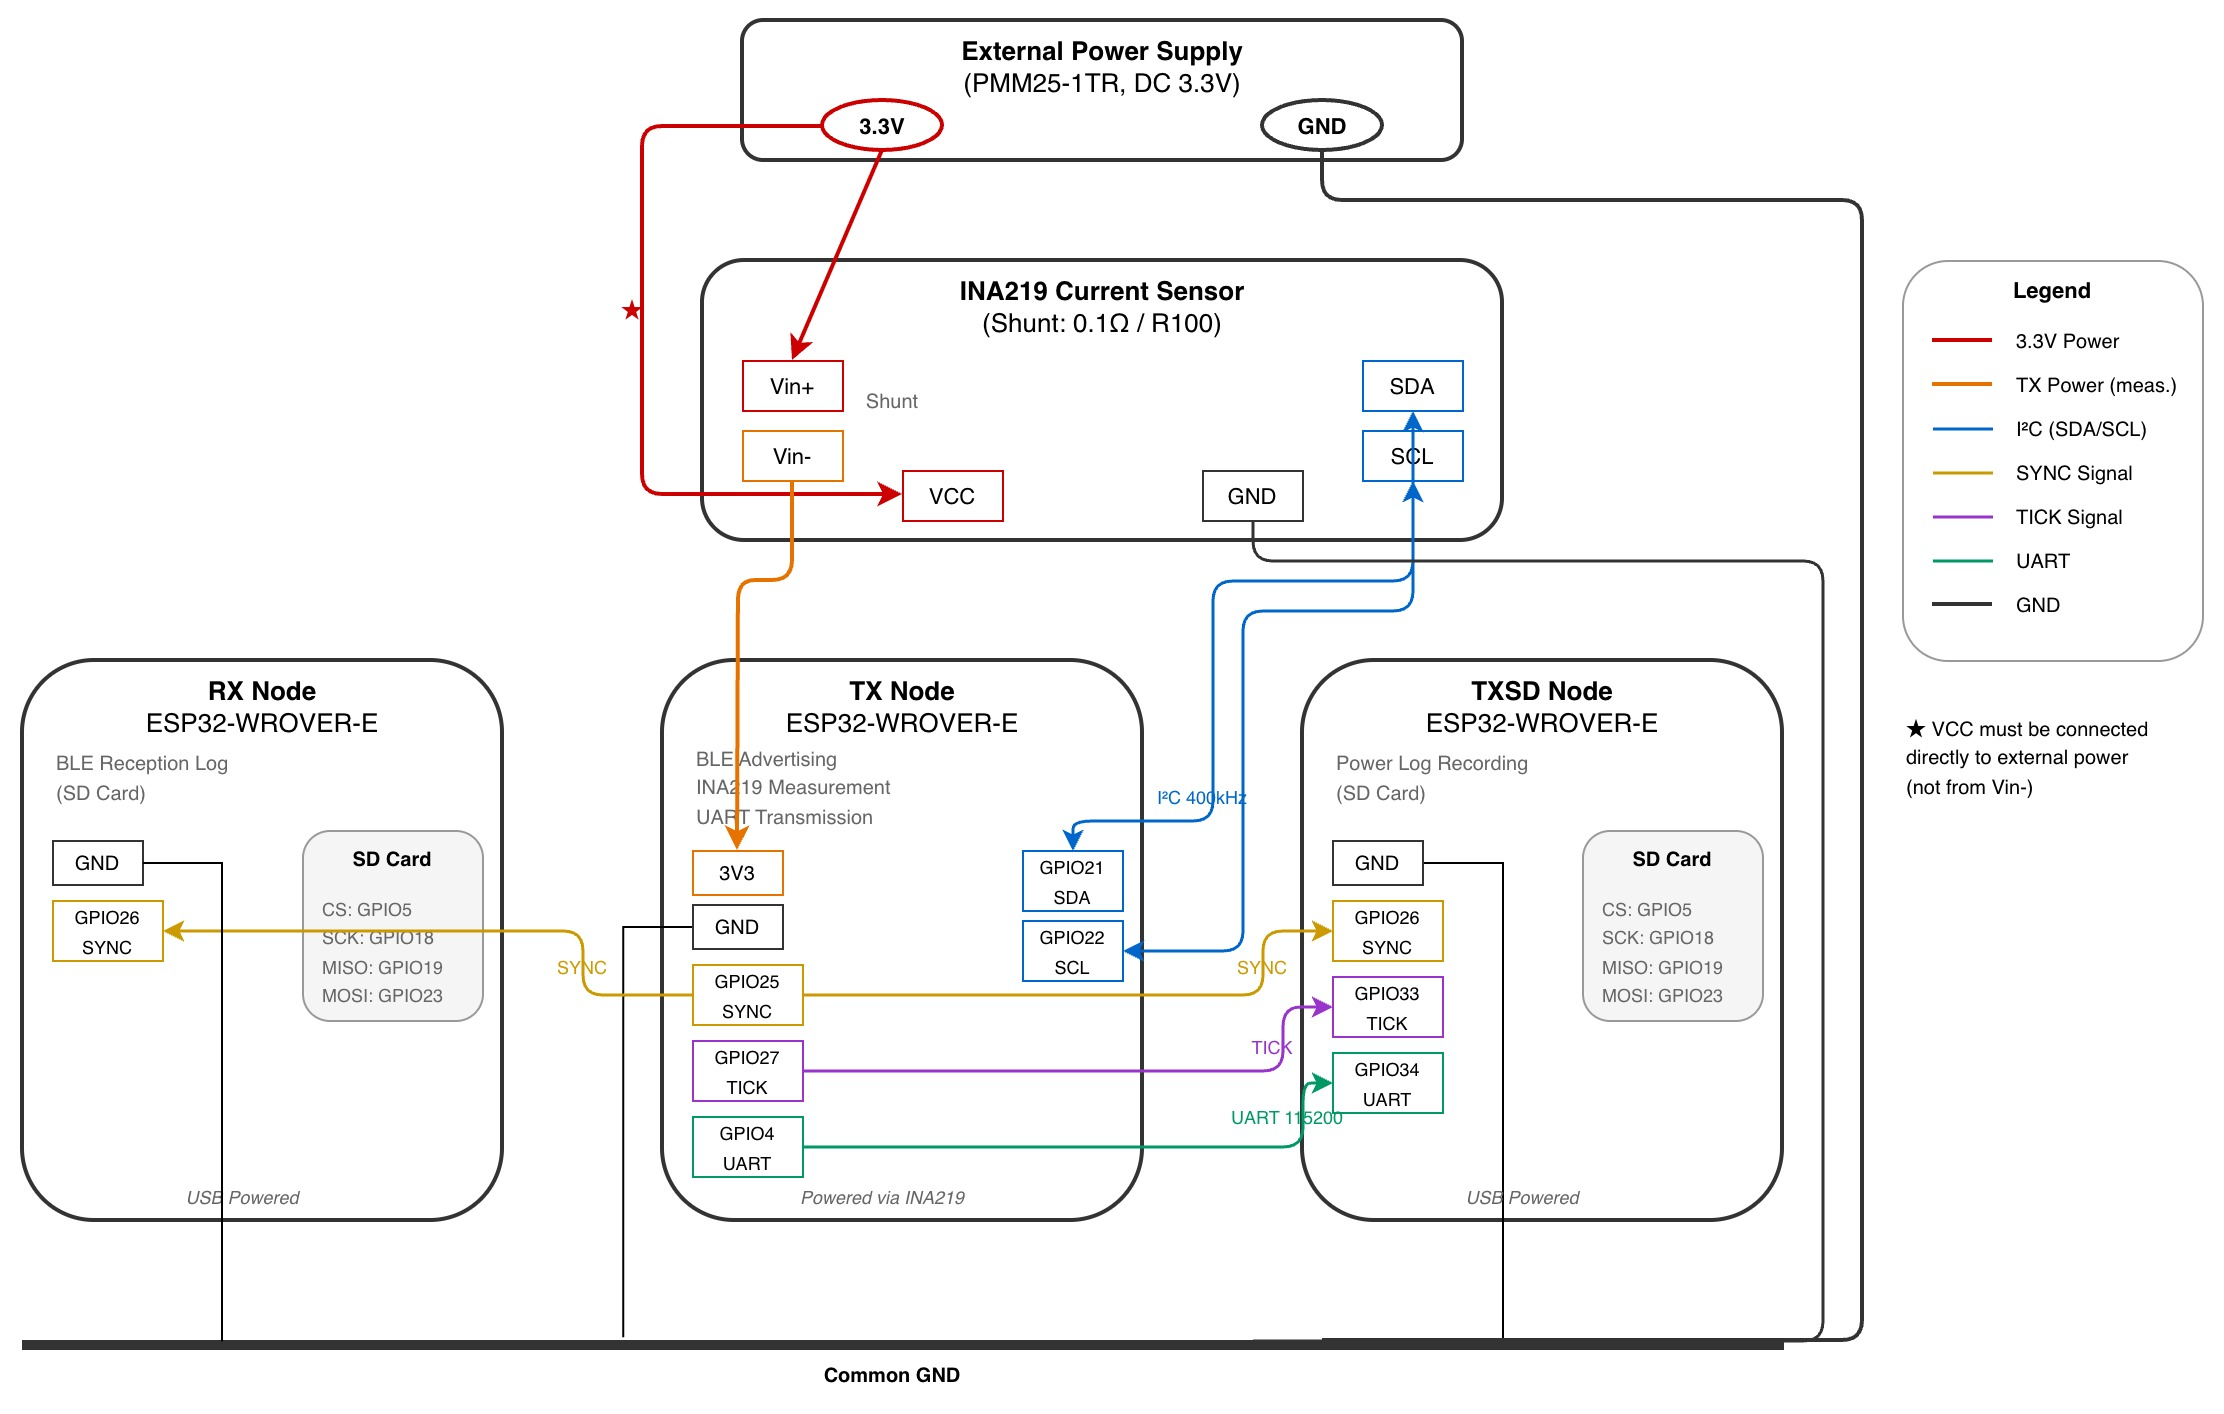
\includegraphics[width=0.9\linewidth]{figures/fig_system_architecture}
  \caption{計測システムの構成}
  \label{fig:system}
\end{figure}

\begin{figure}[t]
  \centering
  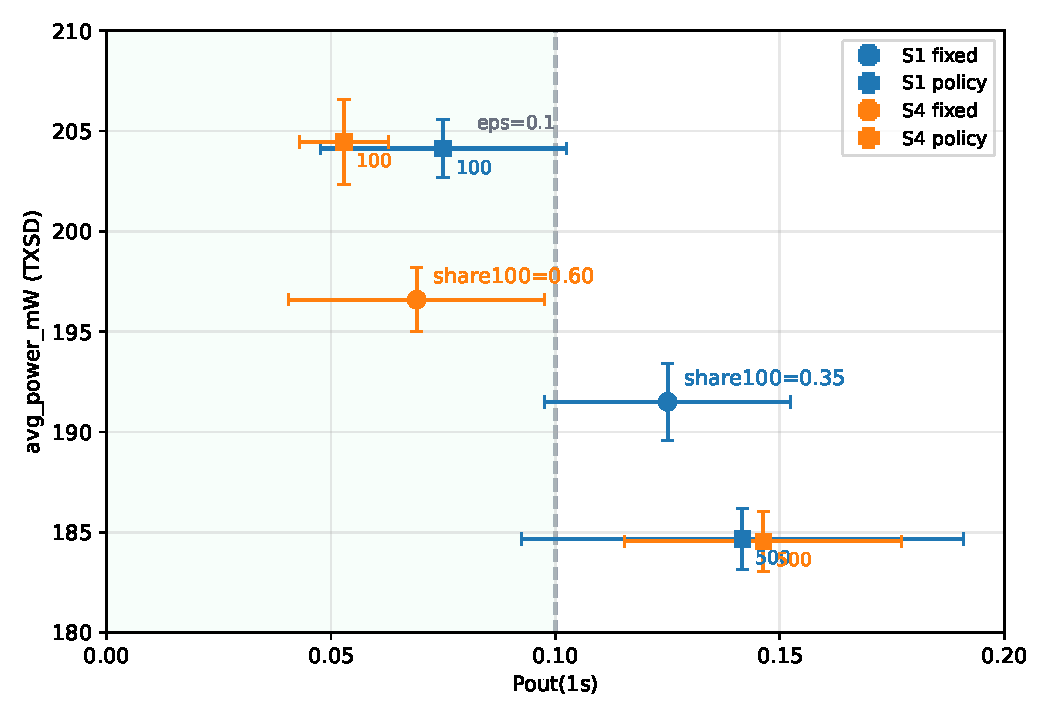
\includegraphics[width=0.9\linewidth]{figures/fig_power_pout}
  \caption{電力と$\Pout(1\mathrm{s})$のトレードオフ（scan90 遷移期）}
  \label{fig:tradeoff}
\end{figure}

\section{実機実験}

\subsection{scan90環境}
\tabref{tab:scan90}にscan90環境（遷移期S4, $n=3$）での結果を示す．
Policyは$\Pout=0.049$，$P=200.6$~mWで，fixed500の$\Pout=0.130$を改善しつつfixed100の$P=208.3$~mWより低電力であった．
share$_{100}$は0.620であり，短間隔を必要な区間に配分できている．
Policyの$TL$平均は1.317~s，PDRは0.448であり，遅延と受信率のバランスが取れている．

\begin{table}[t]
\centering
\footnotesize
\caption{scan90環境（遷移期S4, $n=3$）の実測結果}
\label{tab:scan90}
\begin{tabular}{lccc}
\toprule
条件 & $\Pout(1\mathrm{s})$ & $P$[mW] \\
\midrule
fixed100 & 0.081 & 208.3 \\
fixed500 & 0.130 & 188.1 \\
Policy & 0.049 & 200.6 \\
\bottomrule
\end{tabular}
\end{table}

\subsection{scan70環境}
scan70環境（遷移期S4, $n=3$）では，Policyは$\Pout=0.089$，$P=202.1$~mWであり，fixed500の$\Pout=0.285$に対してQoSを改善しつつfixed100の$P=209.9$~mWより低電力となった．
share$_{100}$は0.618で，遷移期に短間隔が増える傾向を確認した．
Policyの$TL$平均は1.400~sで，fixed500の2.928~sから大きく短縮された．
PDRは0.343であり，低スキャン条件下でも一定の受信率を維持した．

\begin{table}[t]
\centering
\footnotesize
\caption{scan70環境（遷移期S4, $n=3$）の実測結果}
\label{tab:scan70}
\begin{tabular}{lccc}
\toprule
条件 & $\Pout(1\mathrm{s})$ & $P$[mW] \\
\midrule
fixed100 & 0.065 & 209.9 \\
fixed500 & 0.285 & 189.5 \\
Policy & 0.089 & 202.1 \\
\bottomrule
\end{tabular}
\end{table}

\subsection{アブレーション実験}
scan90のS4でCCS-off（$U$のみ）とPolicyを比較すると，$P$は200.6~mW前後でほぼ同等だが，Policyは$\Pout=0.049$とCCS-offの0.065を下回った．
share$_{100}$も0.621付近で同程度であり，$S$を含むCCSがQoS改善に寄与していることが示唆される．
$TL$平均は1.317~sから1.407~sへ悪化するため，$S$の導入は遅延抑制にも有効である．

\section{MABシミュレーション実験}
実機データに基づくデータ駆動型シミュレータを構築し，報酬を消費エネルギー，制約を$\Pout(\tau)$として評価した．
行動集合は500/1000/2000~msとし，高干渉条件（$\tau=1.0$, $\epsilon=0.1$）で比較した．
Safe-UCBとOracleは平均コスト1515.4~mJ/60sかつ違反率0.0で一致し，UCBは平均コスト1078.8~mJ/60sまで低下する一方で違反率0.48156となった．
これにより，制約遵守と省電力のトレードオフが明確になった．

\begin{table}[t]
\centering
\footnotesize
\caption{シミュレーション結果（高干渉条件, $\tau=1.0$, $\epsilon=0.1$）}
\label{tab:sim}
\begin{tabular}{lcc}
\toprule
手法 & 違反率[\%] & 平均コスト[mJ/60s] \\
\midrule
Oracle & 0.00 & 1515.4 \\
Safe-UCB & 0.00 & 1515.4 \\
UCB & 48.16 & 1078.8 \\
\bottomrule
\end{tabular}
\end{table}

\section{おわりに}
実機実験では，CCSに基づく適応制御が固定間隔の極端なトレードオフを緩和し，両環境でQoSと電力の中間運用点を示した．
シミュレーションでは，Safe-UCBが制約内でOracleに近いコストへ到達しうる一方，無制約探索は違反率の増大を招くことが示された．
今後はSafe Contextual Banditのオンライン化と長時間運用でのQoS右裾評価を進める．

\vspace{-2mm}
\section*{参考文献}
\vspace{-1mm}
\printbibliography[heading=none]

\end{document}
